\documentclass[twoside]{book}

% Packages required by doxygen
\usepackage{fixltx2e}
\usepackage{calc}
\usepackage{doxygen}
\usepackage[export]{adjustbox} % also loads graphicx
\usepackage{graphicx}
\usepackage[utf8]{inputenc}
\usepackage{makeidx}
\usepackage{multicol}
\usepackage{multirow}
\PassOptionsToPackage{warn}{textcomp}
\usepackage{textcomp}
\usepackage[nointegrals]{wasysym}
\usepackage[table]{xcolor}

% Font selection
\usepackage[T1]{fontenc}
\usepackage[scaled=.90]{helvet}
\usepackage{courier}
\usepackage{amssymb}
\usepackage{sectsty}
\renewcommand{\familydefault}{\sfdefault}
\allsectionsfont{%
  \fontseries{bc}\selectfont%
  \color{darkgray}%
}
\renewcommand{\DoxyLabelFont}{%
  \fontseries{bc}\selectfont%
  \color{darkgray}%
}
\newcommand{\+}{\discretionary{\mbox{\scriptsize$\hookleftarrow$}}{}{}}

% Page & text layout
\usepackage{geometry}
\geometry{%
  a4paper,%
  top=2.5cm,%
  bottom=2.5cm,%
  left=2.5cm,%
  right=2.5cm%
}
\tolerance=750
\hfuzz=15pt
\hbadness=750
\setlength{\emergencystretch}{15pt}
\setlength{\parindent}{0cm}
\setlength{\parskip}{3ex plus 2ex minus 2ex}
\makeatletter
\renewcommand{\paragraph}{%
  \@startsection{paragraph}{4}{0ex}{-1.0ex}{1.0ex}{%
    \normalfont\normalsize\bfseries\SS@parafont%
  }%
}
\renewcommand{\subparagraph}{%
  \@startsection{subparagraph}{5}{0ex}{-1.0ex}{1.0ex}{%
    \normalfont\normalsize\bfseries\SS@subparafont%
  }%
}
\makeatother

% Headers & footers
\usepackage{fancyhdr}
\pagestyle{fancyplain}
\fancyhead[LE]{\fancyplain{}{\bfseries\thepage}}
\fancyhead[CE]{\fancyplain{}{}}
\fancyhead[RE]{\fancyplain{}{\bfseries\leftmark}}
\fancyhead[LO]{\fancyplain{}{\bfseries\rightmark}}
\fancyhead[CO]{\fancyplain{}{}}
\fancyhead[RO]{\fancyplain{}{\bfseries\thepage}}
\fancyfoot[LE]{\fancyplain{}{}}
\fancyfoot[CE]{\fancyplain{}{}}
\fancyfoot[RE]{\fancyplain{}{\bfseries\scriptsize Generated by Doxygen }}
\fancyfoot[LO]{\fancyplain{}{\bfseries\scriptsize Generated by Doxygen }}
\fancyfoot[CO]{\fancyplain{}{}}
\fancyfoot[RO]{\fancyplain{}{}}
\renewcommand{\footrulewidth}{0.4pt}
\renewcommand{\chaptermark}[1]{%
  \markboth{#1}{}%
}
\renewcommand{\sectionmark}[1]{%
  \markright{\thesection\ #1}%
}

% Indices & bibliography
\usepackage{natbib}
\usepackage[titles]{tocloft}
\setcounter{tocdepth}{3}
\setcounter{secnumdepth}{5}
\makeindex

% Hyperlinks (required, but should be loaded last)
\usepackage{ifpdf}
\ifpdf
  \usepackage[pdftex,pagebackref=true]{hyperref}
\else
  \usepackage[ps2pdf,pagebackref=true]{hyperref}
\fi
\hypersetup{%
  colorlinks=true,%
  linkcolor=blue,%
  citecolor=blue,%
  unicode%
}

% Custom commands
\newcommand{\clearemptydoublepage}{%
  \newpage{\pagestyle{empty}\cleardoublepage}%
}

\usepackage{caption}
\captionsetup{labelsep=space,justification=centering,font={bf},singlelinecheck=off,skip=4pt,position=top}

%===== C O N T E N T S =====

\begin{document}

% Titlepage & ToC
\hypersetup{pageanchor=false,
             bookmarksnumbered=true,
             pdfencoding=unicode
            }
\pagenumbering{alph}
\begin{titlepage}
\vspace*{7cm}
\begin{center}%
{\Large My Project }\\
\vspace*{1cm}
{\large Generated by Doxygen 1.8.13}\\
\end{center}
\end{titlepage}
\clearemptydoublepage
\pagenumbering{roman}
\tableofcontents
\clearemptydoublepage
\pagenumbering{arabic}
\hypersetup{pageanchor=true}

%--- Begin generated contents ---
\chapter{Data Structure Index}
\section{Data Structures}
Here are the data structures with brief descriptions\+:\begin{DoxyCompactList}
\item\contentsline{section}{\hyperlink{structbackground}{background} \\*Struct for background }{\pageref{structbackground}}{}
\end{DoxyCompactList}

\chapter{File Index}
\section{File List}
Here is a list of all documented files with brief descriptions\+:\begin{DoxyCompactList}
\item\contentsline{section}{{\bfseries game.\+h} }{\pageref{game_8h}}{}
\item\contentsline{section}{\hyperlink{haut__bas_8c}{haut\+\_\+bas.\+c} }{\pageref{haut__bas_8c}}{}
\item\contentsline{section}{\hyperlink{main_8c}{main.\+c} \\*Testing Program }{\pageref{main_8c}}{}
\end{DoxyCompactList}

\chapter{Data Structure Documentation}
\hypertarget{structbackground}{}\section{background Struct Reference}
\label{structbackground}\index{background@{background}}


struct for background  




{\ttfamily \#include $<$background.\+h$>$}

\subsection*{Data Fields}
\begin{DoxyCompactItemize}
\item 
S\+D\+L\+\_\+\+Rect \hyperlink{structbackground_a6cd0518c8d8a98207f008f55de18de1d}{bckg}
\item 
S\+D\+L\+\_\+\+Surface $\ast$ \hyperlink{structbackground_a1c5c3a3ebb56924b9f829602f9641006}{img}
\end{DoxyCompactItemize}


\subsection{Detailed Description}
struct for background 

\subsection{Field Documentation}
\mbox{\Hypertarget{structbackground_a6cd0518c8d8a98207f008f55de18de1d}\label{structbackground_a6cd0518c8d8a98207f008f55de18de1d}} 
\index{background@{background}!bckg@{bckg}}
\index{bckg@{bckg}!background@{background}}
\subsubsection{\texorpdfstring{bckg}{bckg}}
{\footnotesize\ttfamily S\+D\+L\+\_\+\+Rect background\+::bckg}

\mbox{\Hypertarget{structbackground_a1c5c3a3ebb56924b9f829602f9641006}\label{structbackground_a1c5c3a3ebb56924b9f829602f9641006}} 
\index{background@{background}!img@{img}}
\index{img@{img}!background@{background}}
\subsubsection{\texorpdfstring{img}{img}}
{\footnotesize\ttfamily S\+D\+L\+\_\+\+Surface$\ast$ background\+::img}



The documentation for this struct was generated from the following file\+:\begin{DoxyCompactItemize}
\item 
\hyperlink{background_8h}{background.\+h}\end{DoxyCompactItemize}

\chapter{File Documentation}
\hypertarget{background_8c}{}\section{background.\+c File Reference}
\label{background_8c}\index{background.\+c@{background.\+c}}
{\ttfamily \#include $<$S\+D\+L/\+S\+D\+L.\+h$>$}\\*
{\ttfamily \#include $<$S\+D\+L/\+S\+D\+L\+\_\+image.\+h$>$}\\*
{\ttfamily \#include \char`\"{}background.\+h\char`\"{}}\\*
Include dependency graph for background.\+c\+:\nopagebreak
\begin{figure}[H]
\begin{center}
\leavevmode
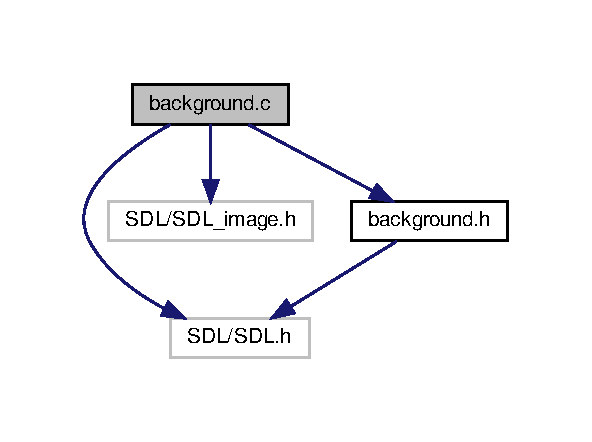
\includegraphics[width=283pt]{background_8c__incl}
\end{center}
\end{figure}
\subsection*{Functions}
\begin{DoxyCompactItemize}
\item 
void \hyperlink{background_8c_a78e1c93646d00d2c16bb3533cf18cf34}{init\+Bckg} (\hyperlink{structbackground}{background} $\ast$b, char url\mbox{[}$\,$\mbox{]})
\begin{DoxyCompactList}\small\item\em To initialize the background b . \end{DoxyCompactList}\item 
void \hyperlink{background_8c_a74cde2d2df1f88fdb2e0ba62193f124c}{show\+Bckg} (S\+D\+L\+\_\+\+Surface $\ast$screen, \hyperlink{structbackground}{background} b)
\begin{DoxyCompactList}\small\item\em To show the background b . \end{DoxyCompactList}\item 
void \hyperlink{background_8c_ae325b42fa1f2e50ce1eb289d21b2a372}{scroll\+To\+Left} (\hyperlink{structbackground}{background} $\ast$b)
\begin{DoxyCompactList}\small\item\em To scroll the background to the left . \end{DoxyCompactList}\item 
void \hyperlink{background_8c_a6ee97702bdd9933893a41c34fa2c2aca}{scroll\+To\+Right} (\hyperlink{structbackground}{background} $\ast$b)
\begin{DoxyCompactList}\small\item\em To scroll the background to the right . \end{DoxyCompactList}\end{DoxyCompactItemize}


\subsection{Detailed Description}
\begin{DoxyAuthor}{Author}
wael 
\end{DoxyAuthor}
\begin{DoxyDate}{Date}
Mai 14, 2020 
\end{DoxyDate}


\subsection{Function Documentation}
\index{background.\+c@{background.\+c}!init\+Bckg@{init\+Bckg}}
\index{init\+Bckg@{init\+Bckg}!background.\+c@{background.\+c}}
\subsubsection[{\texorpdfstring{init\+Bckg(background $\ast$b, char url[])}{initBckg(background *b, char url[])}}]{\setlength{\rightskip}{0pt plus 5cm}void init\+Bckg (
\begin{DoxyParamCaption}
\item[{{\bf background} $\ast$}]{b, }
\item[{char}]{url\mbox{[}$\,$\mbox{]}}
\end{DoxyParamCaption}
)}\hypertarget{background_8c_a78e1c93646d00d2c16bb3533cf18cf34}{}\label{background_8c_a78e1c93646d00d2c16bb3533cf18cf34}


To initialize the background b . 


\begin{DoxyParams}{Parameters}
{\em b} & the background \\
\hline
{\em url} & the url of the image \\
\hline
\end{DoxyParams}
\begin{DoxyReturn}{Returns}
Nothing 
\end{DoxyReturn}
\index{background.\+c@{background.\+c}!scroll\+To\+Left@{scroll\+To\+Left}}
\index{scroll\+To\+Left@{scroll\+To\+Left}!background.\+c@{background.\+c}}
\subsubsection[{\texorpdfstring{scroll\+To\+Left(background $\ast$b)}{scrollToLeft(background *b)}}]{\setlength{\rightskip}{0pt plus 5cm}void scroll\+To\+Left (
\begin{DoxyParamCaption}
\item[{{\bf background} $\ast$}]{b}
\end{DoxyParamCaption}
)}\hypertarget{background_8c_ae325b42fa1f2e50ce1eb289d21b2a372}{}\label{background_8c_ae325b42fa1f2e50ce1eb289d21b2a372}


To scroll the background to the left . 


\begin{DoxyParams}{Parameters}
{\em b} & the background \\
\hline
\end{DoxyParams}
\begin{DoxyReturn}{Returns}
Nothing 
\end{DoxyReturn}
\index{background.\+c@{background.\+c}!scroll\+To\+Right@{scroll\+To\+Right}}
\index{scroll\+To\+Right@{scroll\+To\+Right}!background.\+c@{background.\+c}}
\subsubsection[{\texorpdfstring{scroll\+To\+Right(background $\ast$b)}{scrollToRight(background *b)}}]{\setlength{\rightskip}{0pt plus 5cm}void scroll\+To\+Right (
\begin{DoxyParamCaption}
\item[{{\bf background} $\ast$}]{b}
\end{DoxyParamCaption}
)}\hypertarget{background_8c_a6ee97702bdd9933893a41c34fa2c2aca}{}\label{background_8c_a6ee97702bdd9933893a41c34fa2c2aca}


To scroll the background to the right . 


\begin{DoxyParams}{Parameters}
{\em b} & the background \\
\hline
\end{DoxyParams}
\begin{DoxyReturn}{Returns}
Nothing 
\end{DoxyReturn}
\index{background.\+c@{background.\+c}!show\+Bckg@{show\+Bckg}}
\index{show\+Bckg@{show\+Bckg}!background.\+c@{background.\+c}}
\subsubsection[{\texorpdfstring{show\+Bckg(\+S\+D\+L\+\_\+\+Surface $\ast$screen, background b)}{showBckg(SDL_Surface *screen, background b)}}]{\setlength{\rightskip}{0pt plus 5cm}void show\+Bckg (
\begin{DoxyParamCaption}
\item[{S\+D\+L\+\_\+\+Surface $\ast$}]{screen, }
\item[{{\bf background}}]{b}
\end{DoxyParamCaption}
)}\hypertarget{background_8c_a74cde2d2df1f88fdb2e0ba62193f124c}{}\label{background_8c_a74cde2d2df1f88fdb2e0ba62193f124c}


To show the background b . 


\begin{DoxyParams}{Parameters}
{\em scren} & the screen \\
\hline
{\em b} & the background \\
\hline
\end{DoxyParams}
\begin{DoxyReturn}{Returns}
Nothing 
\end{DoxyReturn}

\hypertarget{background_8h}{}\section{background.\+h File Reference}
\label{background_8h}\index{background.\+h@{background.\+h}}
{\ttfamily \#include $<$S\+D\+L/\+S\+D\+L.\+h$>$}\newline
Include dependency graph for background.\+h\+:
\nopagebreak
\begin{figure}[H]
\begin{center}
\leavevmode
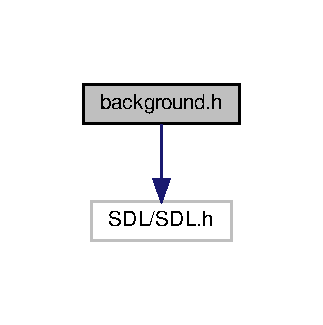
\includegraphics[width=155pt]{background_8h__incl}
\end{center}
\end{figure}
This graph shows which files directly or indirectly include this file\+:
\nopagebreak
\begin{figure}[H]
\begin{center}
\leavevmode
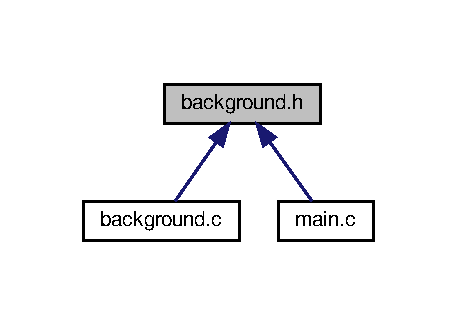
\includegraphics[width=220pt]{background_8h__dep__incl}
\end{center}
\end{figure}
\subsection*{Data Structures}
\begin{DoxyCompactItemize}
\item 
struct \hyperlink{structbackground}{background}
\begin{DoxyCompactList}\small\item\em struct for background \end{DoxyCompactList}\end{DoxyCompactItemize}
\subsection*{Macros}
\begin{DoxyCompactItemize}
\item 
\#define \hyperlink{background_8h_acc99d1c971ce72f6924532f810863aa8}{C\+A\+M\+E\+R\+A\+\_\+W}~100
\item 
\#define \hyperlink{background_8h_ad1e8009af56472a7a1972883b0cca62a}{C\+A\+M\+E\+R\+A\+\_\+H}~200
\end{DoxyCompactItemize}
\subsection*{Typedefs}
\begin{DoxyCompactItemize}
\item 
typedef struct \hyperlink{structbackground}{background} \hyperlink{background_8h_ac7ec97684ccd0aaa88e134ebcc2478bb}{background}
\end{DoxyCompactItemize}
\subsection*{Functions}
\begin{DoxyCompactItemize}
\item 
void \hyperlink{background_8h_a78e1c93646d00d2c16bb3533cf18cf34}{init\+Bckg} (\hyperlink{structbackground}{background} $\ast$b, char url\mbox{[}$\,$\mbox{]})
\begin{DoxyCompactList}\small\item\em To initialize the background b . \end{DoxyCompactList}\item 
void \hyperlink{background_8h_a74cde2d2df1f88fdb2e0ba62193f124c}{show\+Bckg} (S\+D\+L\+\_\+\+Surface $\ast$screen, \hyperlink{structbackground}{background} b)
\item 
void \hyperlink{background_8h_ae325b42fa1f2e50ce1eb289d21b2a372}{scroll\+To\+Left} (\hyperlink{structbackground}{background} $\ast$b)
\item 
void \hyperlink{background_8h_a6ee97702bdd9933893a41c34fa2c2aca}{scroll\+To\+Right} (\hyperlink{structbackground}{background} $\ast$b)
\end{DoxyCompactItemize}


\subsection{Macro Definition Documentation}
\mbox{\Hypertarget{background_8h_ad1e8009af56472a7a1972883b0cca62a}\label{background_8h_ad1e8009af56472a7a1972883b0cca62a}} 
\index{background.\+h@{background.\+h}!C\+A\+M\+E\+R\+A\+\_\+H@{C\+A\+M\+E\+R\+A\+\_\+H}}
\index{C\+A\+M\+E\+R\+A\+\_\+H@{C\+A\+M\+E\+R\+A\+\_\+H}!background.\+h@{background.\+h}}
\subsubsection{\texorpdfstring{C\+A\+M\+E\+R\+A\+\_\+H}{CAMERA\_H}}
{\footnotesize\ttfamily \#define C\+A\+M\+E\+R\+A\+\_\+H~200}

\mbox{\Hypertarget{background_8h_acc99d1c971ce72f6924532f810863aa8}\label{background_8h_acc99d1c971ce72f6924532f810863aa8}} 
\index{background.\+h@{background.\+h}!C\+A\+M\+E\+R\+A\+\_\+W@{C\+A\+M\+E\+R\+A\+\_\+W}}
\index{C\+A\+M\+E\+R\+A\+\_\+W@{C\+A\+M\+E\+R\+A\+\_\+W}!background.\+h@{background.\+h}}
\subsubsection{\texorpdfstring{C\+A\+M\+E\+R\+A\+\_\+W}{CAMERA\_W}}
{\footnotesize\ttfamily \#define C\+A\+M\+E\+R\+A\+\_\+W~100}



\subsection{Typedef Documentation}
\mbox{\Hypertarget{background_8h_ac7ec97684ccd0aaa88e134ebcc2478bb}\label{background_8h_ac7ec97684ccd0aaa88e134ebcc2478bb}} 
\index{background.\+h@{background.\+h}!background@{background}}
\index{background@{background}!background.\+h@{background.\+h}}
\subsubsection{\texorpdfstring{background}{background}}
{\footnotesize\ttfamily typedef struct \hyperlink{structbackground}{background} \hyperlink{structbackground}{background}}



\subsection{Function Documentation}
\mbox{\Hypertarget{background_8h_a78e1c93646d00d2c16bb3533cf18cf34}\label{background_8h_a78e1c93646d00d2c16bb3533cf18cf34}} 
\index{background.\+h@{background.\+h}!init\+Bckg@{init\+Bckg}}
\index{init\+Bckg@{init\+Bckg}!background.\+h@{background.\+h}}
\subsubsection{\texorpdfstring{init\+Bckg()}{initBckg()}}
{\footnotesize\ttfamily void init\+Bckg (\begin{DoxyParamCaption}\item[{\hyperlink{structbackground}{background} $\ast$}]{b,  }\item[{char}]{url\mbox{[}$\,$\mbox{]} }\end{DoxyParamCaption})}



To initialize the background b . 


\begin{DoxyParams}{Parameters}
{\em b} & the background \\
\hline
{\em url} & the url of the image \\
\hline
\end{DoxyParams}
\begin{DoxyReturn}{Returns}
Nothing 
\end{DoxyReturn}
Here is the caller graph for this function\+:
\nopagebreak
\begin{figure}[H]
\begin{center}
\leavevmode
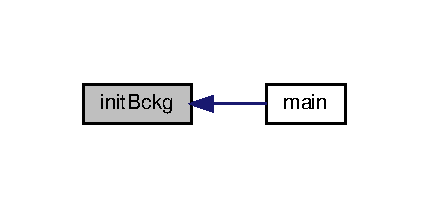
\includegraphics[width=206pt]{background_8h_a78e1c93646d00d2c16bb3533cf18cf34_icgraph}
\end{center}
\end{figure}
\mbox{\Hypertarget{background_8h_ae325b42fa1f2e50ce1eb289d21b2a372}\label{background_8h_ae325b42fa1f2e50ce1eb289d21b2a372}} 
\index{background.\+h@{background.\+h}!scroll\+To\+Left@{scroll\+To\+Left}}
\index{scroll\+To\+Left@{scroll\+To\+Left}!background.\+h@{background.\+h}}
\subsubsection{\texorpdfstring{scroll\+To\+Left()}{scrollToLeft()}}
{\footnotesize\ttfamily void scroll\+To\+Left (\begin{DoxyParamCaption}\item[{\hyperlink{structbackground}{background} $\ast$}]{b }\end{DoxyParamCaption})}

Here is the caller graph for this function\+:
\nopagebreak
\begin{figure}[H]
\begin{center}
\leavevmode
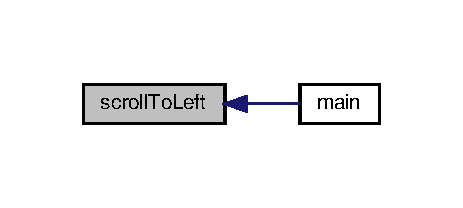
\includegraphics[width=222pt]{background_8h_ae325b42fa1f2e50ce1eb289d21b2a372_icgraph}
\end{center}
\end{figure}
\mbox{\Hypertarget{background_8h_a6ee97702bdd9933893a41c34fa2c2aca}\label{background_8h_a6ee97702bdd9933893a41c34fa2c2aca}} 
\index{background.\+h@{background.\+h}!scroll\+To\+Right@{scroll\+To\+Right}}
\index{scroll\+To\+Right@{scroll\+To\+Right}!background.\+h@{background.\+h}}
\subsubsection{\texorpdfstring{scroll\+To\+Right()}{scrollToRight()}}
{\footnotesize\ttfamily void scroll\+To\+Right (\begin{DoxyParamCaption}\item[{\hyperlink{structbackground}{background} $\ast$}]{b }\end{DoxyParamCaption})}

Here is the caller graph for this function\+:
\nopagebreak
\begin{figure}[H]
\begin{center}
\leavevmode
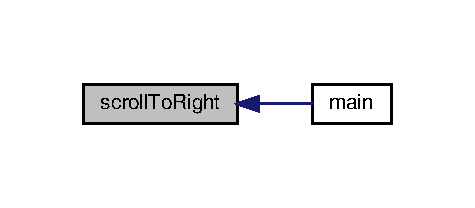
\includegraphics[width=228pt]{background_8h_a6ee97702bdd9933893a41c34fa2c2aca_icgraph}
\end{center}
\end{figure}
\mbox{\Hypertarget{background_8h_a74cde2d2df1f88fdb2e0ba62193f124c}\label{background_8h_a74cde2d2df1f88fdb2e0ba62193f124c}} 
\index{background.\+h@{background.\+h}!show\+Bckg@{show\+Bckg}}
\index{show\+Bckg@{show\+Bckg}!background.\+h@{background.\+h}}
\subsubsection{\texorpdfstring{show\+Bckg()}{showBckg()}}
{\footnotesize\ttfamily void show\+Bckg (\begin{DoxyParamCaption}\item[{S\+D\+L\+\_\+\+Surface $\ast$}]{screen,  }\item[{\hyperlink{structbackground}{background}}]{b }\end{DoxyParamCaption})}

Here is the caller graph for this function\+:
\nopagebreak
\begin{figure}[H]
\begin{center}
\leavevmode
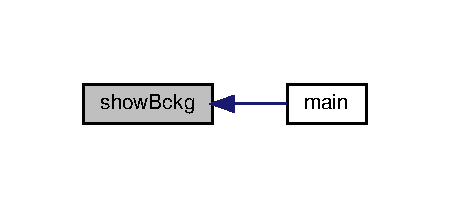
\includegraphics[width=216pt]{background_8h_a74cde2d2df1f88fdb2e0ba62193f124c_icgraph}
\end{center}
\end{figure}

\hypertarget{main_8c}{}\section{main.\+c File Reference}
\label{main_8c}\index{main.\+c@{main.\+c}}
{\ttfamily \#include $<$stdlib.\+h$>$}\\*
{\ttfamily \#include $<$stdio.\+h$>$}\\*
{\ttfamily \#include $<$S\+D\+L/\+S\+D\+L.\+h$>$}\\*
{\ttfamily \#include $<$S\+D\+L/\+S\+D\+L\+\_\+image.\+h$>$}\\*
{\ttfamily \#include \char`\"{}background.\+h\char`\"{}}\\*
Include dependency graph for main.\+c\+:\nopagebreak
\begin{figure}[H]
\begin{center}
\leavevmode
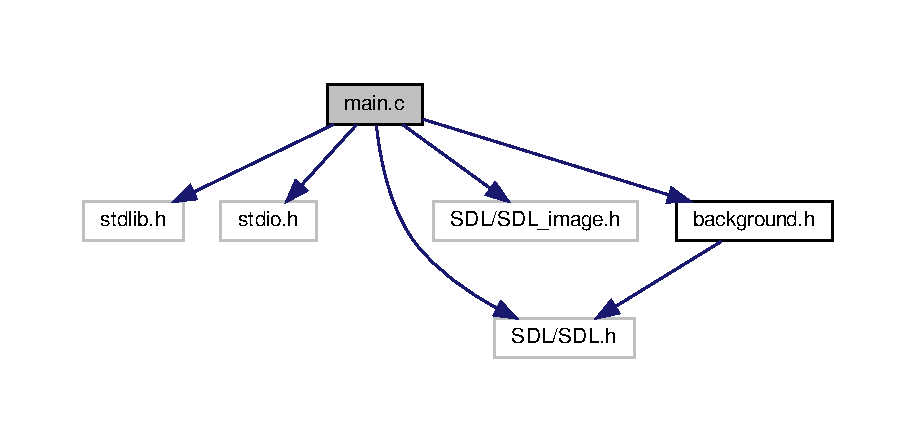
\includegraphics[width=350pt]{main_8c__incl}
\end{center}
\end{figure}
\subsection*{Functions}
\begin{DoxyCompactItemize}
\item 
int {\bfseries main} (int argc, char $\ast$argv\mbox{[}$\,$\mbox{]})\hypertarget{main_8c_a0ddf1224851353fc92bfbff6f499fa97}{}\label{main_8c_a0ddf1224851353fc92bfbff6f499fa97}

\end{DoxyCompactItemize}


\subsection{Detailed Description}
\begin{DoxyAuthor}{Author}
wael 
\end{DoxyAuthor}
\begin{DoxyDate}{Date}
Mai 14, 2020 
\end{DoxyDate}

%--- End generated contents ---

% Index
\backmatter
\newpage
\phantomsection
\clearemptydoublepage
\addcontentsline{toc}{chapter}{Index}
\printindex

\end{document}
